% Options for packages loaded elsewhere
\PassOptionsToPackage{unicode}{hyperref}
\PassOptionsToPackage{hyphens}{url}
%
\documentclass[
  letterpaper,
]{book}

\usepackage{amsmath,amssymb}
\usepackage{lmodern}
\usepackage{iftex}
\ifPDFTeX
  \usepackage[T1]{fontenc}
  \usepackage[utf8]{inputenc}
  \usepackage{textcomp} % provide euro and other symbols
\else % if luatex or xetex
  \usepackage{unicode-math}
  \defaultfontfeatures{Scale=MatchLowercase}
  \defaultfontfeatures[\rmfamily]{Ligatures=TeX,Scale=1}
\fi
% Use upquote if available, for straight quotes in verbatim environments
\IfFileExists{upquote.sty}{\usepackage{upquote}}{}
\IfFileExists{microtype.sty}{% use microtype if available
  \usepackage[]{microtype}
  \UseMicrotypeSet[protrusion]{basicmath} % disable protrusion for tt fonts
}{}
\makeatletter
\@ifundefined{KOMAClassName}{% if non-KOMA class
  \IfFileExists{parskip.sty}{%
    \usepackage{parskip}
  }{% else
    \setlength{\parindent}{0pt}
    \setlength{\parskip}{6pt plus 2pt minus 1pt}}
}{% if KOMA class
  \KOMAoptions{parskip=half}}
\makeatother
\usepackage{xcolor}
\setlength{\emergencystretch}{3em} % prevent overfull lines
\setcounter{secnumdepth}{5}
% Make \paragraph and \subparagraph free-standing
\ifx\paragraph\undefined\else
  \let\oldparagraph\paragraph
  \renewcommand{\paragraph}[1]{\oldparagraph{#1}\mbox{}}
\fi
\ifx\subparagraph\undefined\else
  \let\oldsubparagraph\subparagraph
  \renewcommand{\subparagraph}[1]{\oldsubparagraph{#1}\mbox{}}
\fi


\providecommand{\tightlist}{%
  \setlength{\itemsep}{0pt}\setlength{\parskip}{0pt}}\usepackage{longtable,booktabs,array}
\usepackage{calc} % for calculating minipage widths
% Correct order of tables after \paragraph or \subparagraph
\usepackage{etoolbox}
\makeatletter
\patchcmd\longtable{\par}{\if@noskipsec\mbox{}\fi\par}{}{}
\makeatother
% Allow footnotes in longtable head/foot
\IfFileExists{footnotehyper.sty}{\usepackage{footnotehyper}}{\usepackage{footnote}}
\makesavenoteenv{longtable}
\usepackage{graphicx}
\makeatletter
\def\maxwidth{\ifdim\Gin@nat@width>\linewidth\linewidth\else\Gin@nat@width\fi}
\def\maxheight{\ifdim\Gin@nat@height>\textheight\textheight\else\Gin@nat@height\fi}
\makeatother
% Scale images if necessary, so that they will not overflow the page
% margins by default, and it is still possible to overwrite the defaults
% using explicit options in \includegraphics[width, height, ...]{}
\setkeys{Gin}{width=\maxwidth,height=\maxheight,keepaspectratio}
% Set default figure placement to htbp
\makeatletter
\def\fps@figure{htbp}
\makeatother

\makeatletter
\makeatother
\makeatletter
\@ifpackageloaded{bookmark}{}{\usepackage{bookmark}}
\makeatother
\makeatletter
\@ifpackageloaded{caption}{}{\usepackage{caption}}
\AtBeginDocument{%
\ifdefined\contentsname
  \renewcommand*\contentsname{Table of contents}
\else
  \newcommand\contentsname{Table of contents}
\fi
\ifdefined\listfigurename
  \renewcommand*\listfigurename{List of Figures}
\else
  \newcommand\listfigurename{List of Figures}
\fi
\ifdefined\listtablename
  \renewcommand*\listtablename{List of Tables}
\else
  \newcommand\listtablename{List of Tables}
\fi
\ifdefined\figurename
  \renewcommand*\figurename{Figure}
\else
  \newcommand\figurename{Figure}
\fi
\ifdefined\tablename
  \renewcommand*\tablename{Table}
\else
  \newcommand\tablename{Table}
\fi
}
\@ifpackageloaded{float}{}{\usepackage{float}}
\floatstyle{ruled}
\@ifundefined{c@chapter}{\newfloat{codelisting}{h}{lop}}{\newfloat{codelisting}{h}{lop}[chapter]}
\floatname{codelisting}{Listing}
\newcommand*\listoflistings{\listof{codelisting}{List of Listings}}
\makeatother
\makeatletter
\@ifpackageloaded{caption}{}{\usepackage{caption}}
\@ifpackageloaded{subcaption}{}{\usepackage{subcaption}}
\makeatother
\makeatletter
\@ifpackageloaded{tcolorbox}{}{\usepackage[many]{tcolorbox}}
\makeatother
\makeatletter
\@ifundefined{shadecolor}{\definecolor{shadecolor}{rgb}{.97, .97, .97}}
\makeatother
\makeatletter
\makeatother
\ifLuaTeX
  \usepackage{selnolig}  % disable illegal ligatures
\fi
\IfFileExists{bookmark.sty}{\usepackage{bookmark}}{\usepackage{hyperref}}
\IfFileExists{xurl.sty}{\usepackage{xurl}}{} % add URL line breaks if available
\urlstyle{same} % disable monospaced font for URLs
\hypersetup{
  pdftitle={Experimental Books Workshop Catalogue},
  pdfauthor={Experimental books conference participants},
  hidelinks,
  pdfcreator={LaTeX via pandoc}}

\title{Experimental Books Workshop Catalogue}
\author{Experimental books conference participants}
\date{2/20/23}

\begin{document}
\frontmatter
\maketitle
\ifdefined\Shaded\renewenvironment{Shaded}{\begin{tcolorbox}[enhanced, boxrule=0pt, interior hidden, borderline west={3pt}{0pt}{shadecolor}, sharp corners, breakable, frame hidden]}{\end{tcolorbox}}\fi

\renewcommand*\contentsname{Table of contents}
{
\setcounter{tocdepth}{2}
\tableofcontents
}
\mainmatter
\bookmarksetup{startatroot}

\hypertarget{workshop-programme-publishing-from-collections-introducing-computational-publishing-for-culture}{%
\chapter{Workshop Programme: Publishing from Collections: Introducing
Computational Publishing for
Culture}\label{workshop-programme-publishing-from-collections-introducing-computational-publishing-for-culture}}

\href{https://mrchristian.github.io/Workshop-Publishing-from-Collections/}{Programme
instructions}

2023-02-20 v1.0

Experimental Books -- Re-imagining Scholarly Publishing, COPIM. Workshop
URL: https://experimentalbooks.pubpub.org/programme-overview

Contribution from Task Area 4 of the
\href{https://nfdi4culture.de/}{NFDI4Culture} is looking at which
initiatives are enhancing their publications for open scholarship. Its
aim is to establish a guideline for scholars to create publications and
their associated data with a focus on long-term digital preservation.

Example workshop publication:
\href{https://simonxix.github.io/Experimental_Books_workshop/}{toc
Baroque /toc}

\hypertarget{cite-as}{%
\subsection{Cite as~}\label{cite-as}}

Document DOI:
\href{https://doi.org/10.5281/zenodo.7652524}{10.5281/zenodo.7652524}
\textbar{} Author: Simon Worthington
https://orcid.org/0000-0002-8579-9717

This work is licensed under a Creative Commons Attribution-ShareAlike
4.0 International License.

Book cover: Reworking of
\href{https://en.wikipedia.org/wiki/File:Pendant_in_the_form_of_a_siren_MET_DT7173.jpg}{Baroque
pearl with enamelled gold mounts set with rubies}. Creative Commons CC0
1.0 Universal Public Domain Dedication. This file was donated to
Wikimedia Commons as part of a project by the Metropolitan Museum of
Art.

\bookmarksetup{startatroot}

\hypertarget{activity-a-paintings-catalogue-in-jupyter-notebook}{%
\chapter{Activity A: Paintings catalogue in Jupyter
Notebook}\label{activity-a-paintings-catalogue-in-jupyter-notebook}}

Objective: Make a selection of nine paintings for the exhibition
catalogue to be selected from Wikidata and rendered multi-format in
Quarto.

The below Python code uses SPARQLWrapper to retrieve data from Wikidata
based on a SPARQL query.

Wikidata link: \url{http://www.wikidata.org/entity/Q29474642}

Title: The Birth of Benjamin

Year: 1650

Creator: Francesco Furini

Copyright: public domain

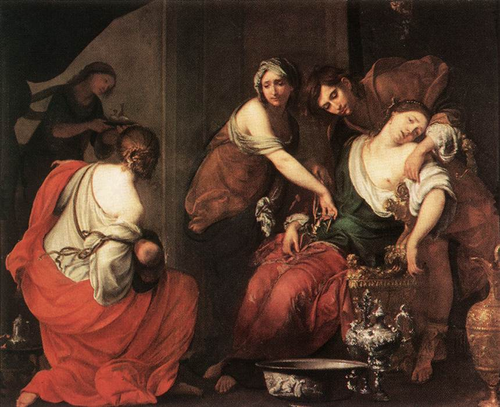
\includegraphics{./paintings_files/figure-pdf/cell-2-output-2.png}

Wikidata link: \url{http://www.wikidata.org/entity/Q29474649}

Title: A Cynical Philosopher

Year: 1650

Creator: Luca Giordano

Copyright: public domain

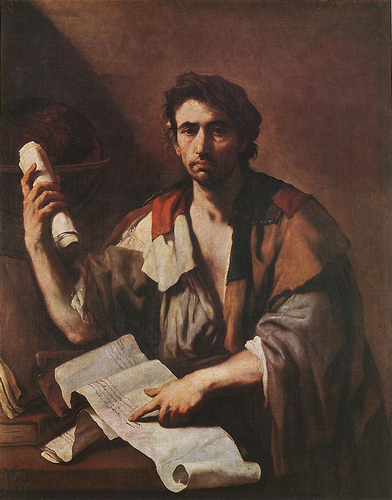
\includegraphics{./paintings_files/figure-pdf/cell-2-output-4.png}

Wikidata link: \url{http://www.wikidata.org/entity/Q29474651}

Title: Solomon and the Queen of Sheba

Year: 1697

Creator: Luca Giordano

Copyright: public domain

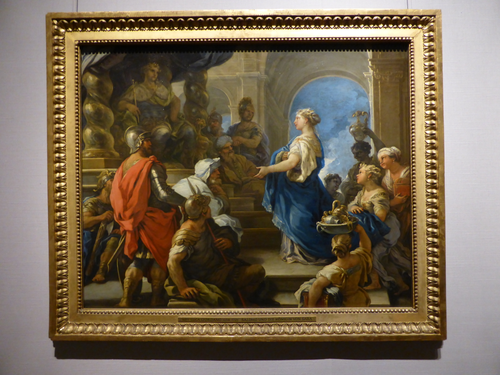
\includegraphics{./paintings_files/figure-pdf/cell-2-output-6.png}

Wikidata link: \url{http://www.wikidata.org/entity/Q29477235}

Title: Q29477235

Year: 1674

Creator: Antonio Triva

Copyright: public domain

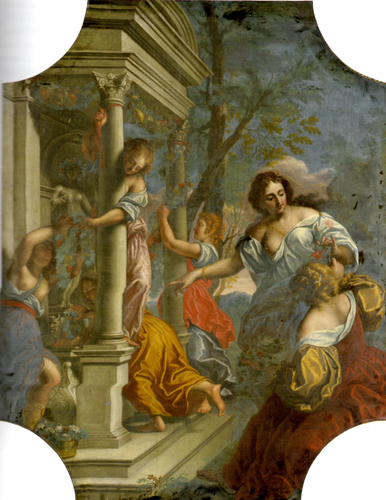
\includegraphics{./paintings_files/figure-pdf/cell-2-output-8.png}

Wikidata link: \url{http://www.wikidata.org/entity/Q29477863}

Title: Q29477863

Year: 1633

Creator: Guido Reni

Copyright: public domain

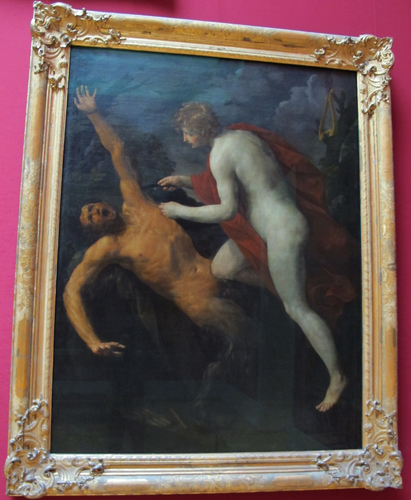
\includegraphics{./paintings_files/figure-pdf/cell-2-output-10.png}

Wikidata link: \url{http://www.wikidata.org/entity/Q29477898}

Title: Still-Life with Books

Year: 1628

Creator: Jan Lievens

Copyright: public domain

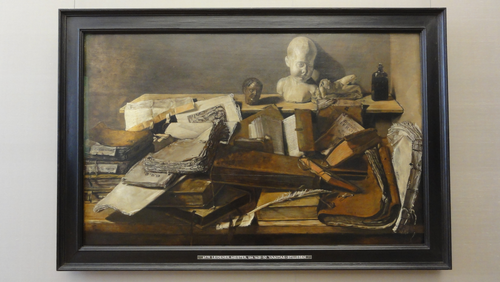
\includegraphics{./paintings_files/figure-pdf/cell-2-output-12.png}

Wikidata link: \url{http://www.wikidata.org/entity/Q29480557}

Title: Feast of Herod

Year: 1630

Creator:
http://www.wikidata.org/.well-known/genid/3f945710e81609ba4bae458b2820460a

Copyright: public domain

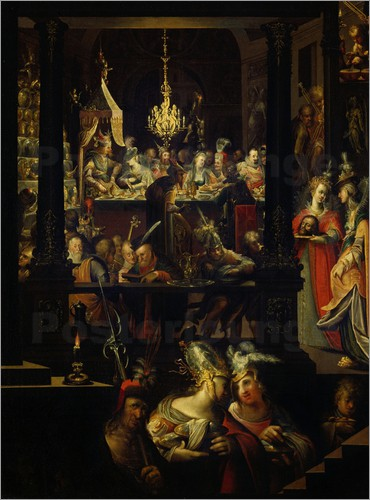
\includegraphics{./paintings_files/figure-pdf/cell-2-output-14.png}

Wikidata link: \url{http://www.wikidata.org/entity/Q29480565}

Title: Venus and Cupid

Year: 1625

Creator: Heinrich Bollandt

Copyright: public domain

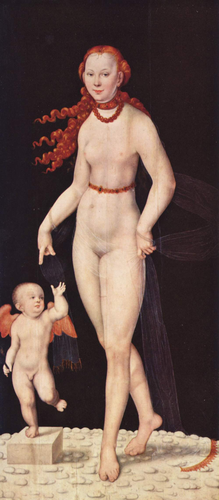
\includegraphics{./paintings_files/figure-pdf/cell-2-output-16.png}

Wikidata link: \url{http://www.wikidata.org/entity/Q29480594}

Title: Still-life with Parrot

Year: 1630

Creator: Georg Flegel

Copyright: public domain

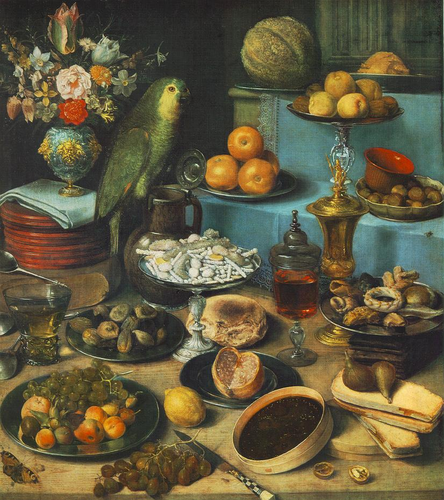
\includegraphics{./paintings_files/figure-pdf/cell-2-output-18.png}

\bookmarksetup{startatroot}

\hypertarget{activity-b-embedded-video-in-jupyter-notebook}{%
\chapter{Activity B: Embedded video in Jupyter
Notebook}\label{activity-b-embedded-video-in-jupyter-notebook}}

Objective: Running and editing Juypter Notebooks in MyBinder and
retrieving video and 3D models as embeds.

The below Python code experiments with retrieving video data via iframe
embedding.

\begin{verbatim}
<IPython.core.display.HTML object>
\end{verbatim}

\hypertarget{d-model-embedding}{%
\section{3D model embedding}\label{d-model-embedding}}

The below Python code experiments with retrieving 3D data via iframe
embedding.

\begin{verbatim}
<IPython.core.display.HTML object>
\end{verbatim}

\begin{verbatim}
<IPython.core.display.HTML object>
\end{verbatim}

\bookmarksetup{startatroot}

\hypertarget{nextcloud-md-editor}{%
\chapter{NextCloud MD Editor}\label{nextcloud-md-editor}}

Call outs?

\begin{figure}

{\centering 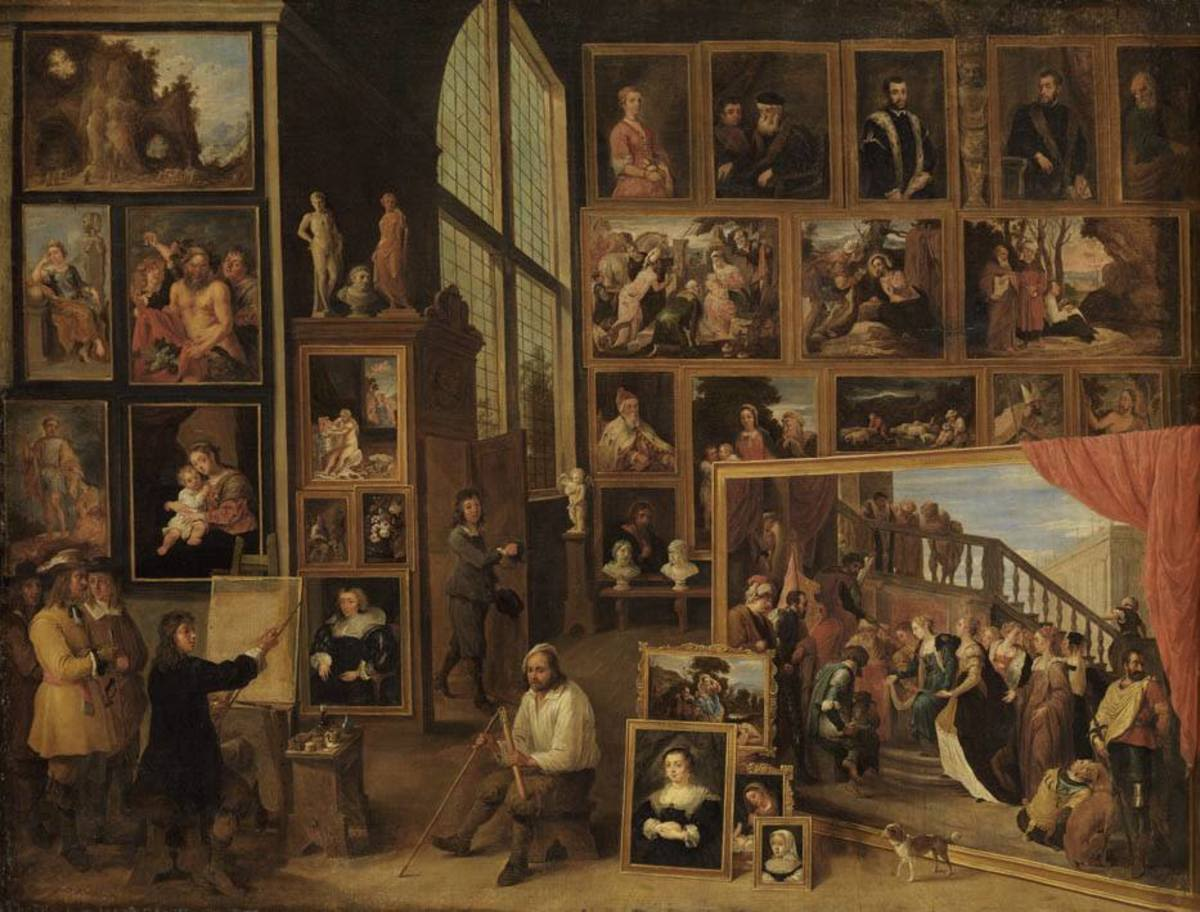
\includegraphics{./6780765/Brussels.jpg}

}

\caption{David\_Teniers\_(II)\_-\_The\_gallery\_of\_Archduke\_Leopold\_in\_Brussels.jpg}

\end{figure}

\begin{longtable}[]{@{}llll@{}}
\toprule()
Vegetables & Not vegetables & Bier & Wein \\
\midrule()
\endhead
Raddish & Mushroom & & \\
Leak & & & \\
\bottomrule()
\end{longtable}

Please edit here: hello here is nils

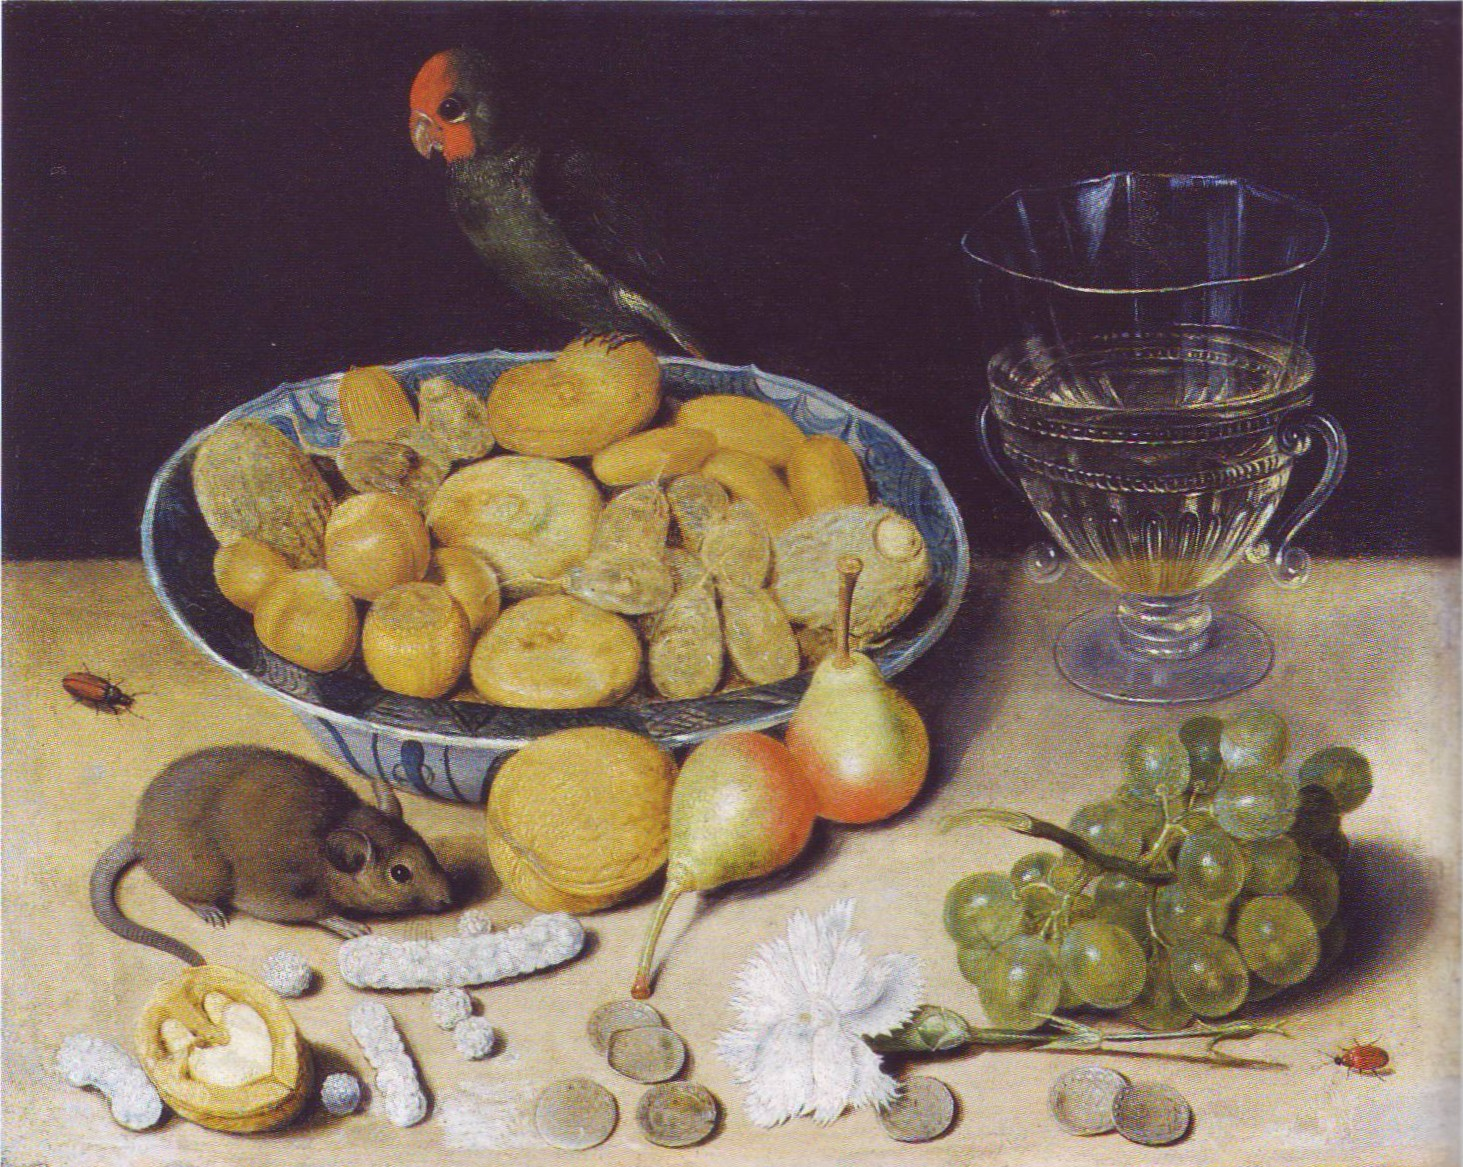
\includegraphics{./6780765/Papagei.jpg}\\
\textbf{English:} \emph{Still-life with Parrot}

\textbf{Deutsch:} \emph{Stillleben mit Papagei}

\emph{to do list}

\begin{itemize}
\tightlist
\item[$\square$]
  \emph{Activity 1}
\item[$\square$]
  Activity 2
\item[$\square$]
  Activity 3
\end{itemize}

Sucess

Warning

Danger

and this is paul, look I can make edits!!

SW: Ive tuurned on the colour marking for users, but this maybe only
shows up for me and not all other users.

nils: at the moment i dont see any color marking =\textgreater{} fixed
by enable option

The colour thing must be user specific.

\begin{verbatim}
WHERE
{
  # find items which:
  # are instances of (wdt:P31) paintings (wd:Q3305213)
  # have the property (wdt:P195) of being in collection wd:Q812285 (Bavarian State Painting Collections https://www.wikidata.org/wiki/Wikidata:WikiProject_sum_of_all_paintings/Collection/Bavarian_State_Painting_Collections)
  ?item wdt:P31 wd:Q3305213 .
  ?item wdt:P195 wd:Q812285 .
  # get the item's creator property (wdt:P170)
  ?item wdt:P170 ?creator .
  # get the item's image property (wdt:P18)
  ?item wdt:P18 ?image .
  # get the item's copyright status (wdt:P6216)
  ?item wdt:P6216 ?copyright . 
    {
    ?item wdt:P571 ?inception.
    BIND(YEAR(?inception) AS ?inceptionyear)
  }
\end{verbatim}

\bookmarksetup{startatroot}

\hypertarget{end}{%
\chapter{END}\label{end}}

\begin{center}\rule{0.5\linewidth}{0.5pt}\end{center}

\bookmarksetup{startatroot}

\hypertarget{baroque-ai}{%
\chapter{Baroque \#AI}\label{baroque-ai}}

\hypertarget{series-baroque-toc}{%
\section{Series: Baroque TOC}\label{series-baroque-toc}}

Publication: An exhibition catalogue

Project goal and activities:

The goal is to create a finished exhibition catalogue - like so:

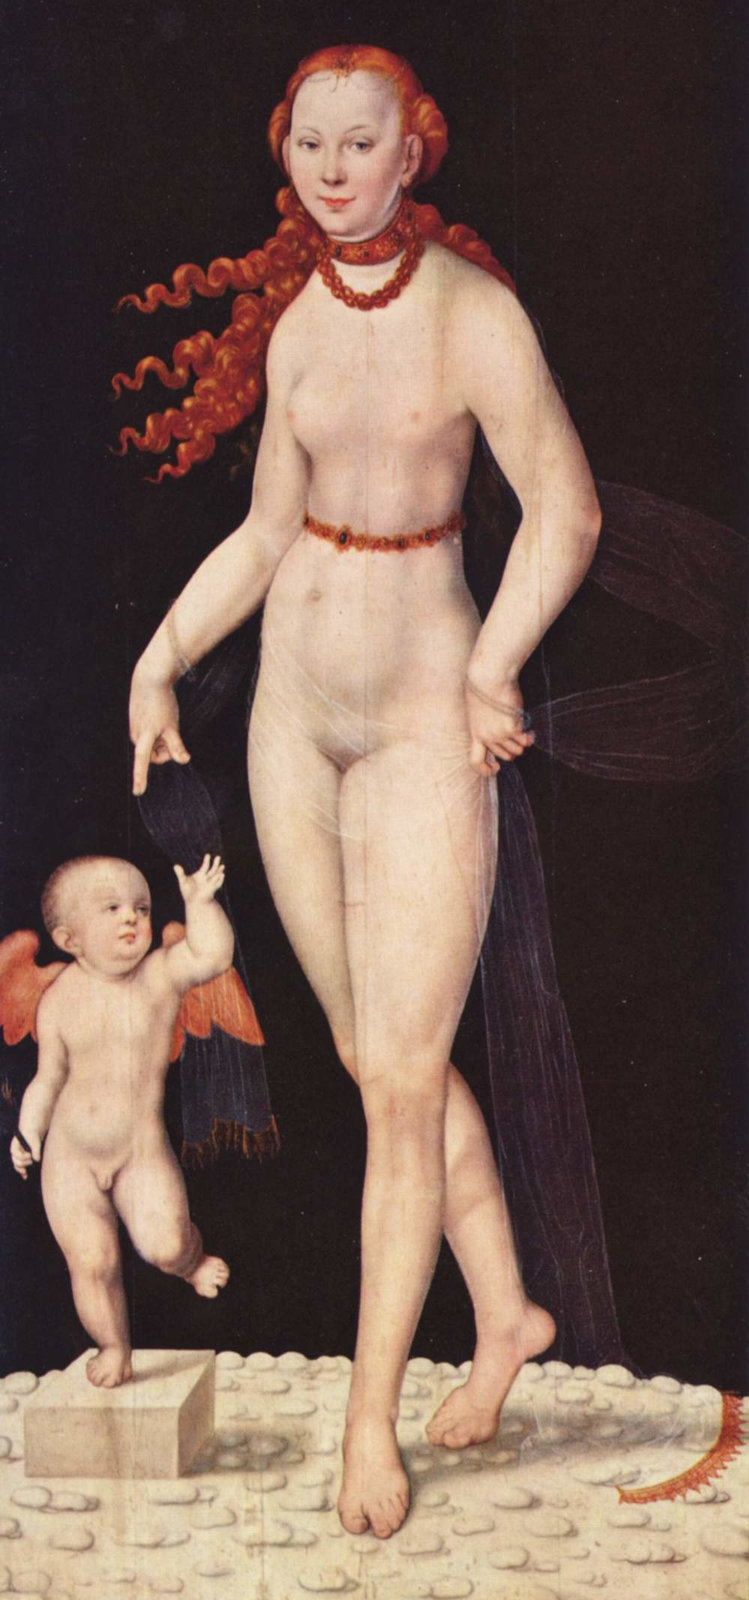
\includegraphics{./6780765/Cupido.jpg}Heinrich Bollandt - Venus und
Cupido, between circa 1620 and circa 1630
\url{https://commons.wikimedia.org/wiki/File:Heinrich_Bollandt_-_Venus_und_Cupido.jpg}

\hypertarget{activities}{%
\section{Activities}\label{activities}}

\hypertarget{markup-testing}{%
\section{Markup testing}\label{markup-testing}}

Headers

\bookmarksetup{startatroot}

\hypertarget{header-1}{%
\chapter{Header 1}\label{header-1}}

\hypertarget{header-2}{%
\section{Header 2}\label{header-2}}

\hypertarget{header-3}{%
\subsection{Header 3}\label{header-3}}

\hypertarget{header-4}{%
\subsubsection{Header 4}\label{header-4}}

\hypertarget{header-5}{%
\paragraph{Header 5}\label{header-5}}

\hypertarget{header-6}{%
\subparagraph{Header 6}\label{header-6}}


\backmatter

\end{document}
